\documentclass[11pt]{article}
\usepackage[a4paper,margin=2cm]{geometry}
\usepackage{physics}
\usepackage{amsmath,amssymb}
\usepackage{graphicx}
\usepackage{import}
\usepackage{standalone}
\begin{document}
\title{Quantum Computation}
\maketitle
\section*{Notation}
\begin{description}
    \item [State] $\ket{\alpha}$
    \item [Dual Vector] $\bra{\alpha}$
    \item [Hibert Space] $\mathcal{H}$
    \item [Computational Basis] \hfill
    \begin{itemize}
        \item $\ket{0}$
        \item $\ket{1}$
        \item $\ket{2}$ etc.
    \end{itemize}
\end{description}
\section{Elementary Concepts}
A state $\ket{\alpha}$ is a vector in a Hilbert space $\mathcal{H}$. The smallest non-trvial space is $\mathbf{C}^{2}$, with two basis states. The most common basis choice is called `computational', which has matrix representaiton
\begin{align*}
    \ket{0} = \begin{pmatrix}
                    1 \\
                    0 \\
                \end{pmatrix} \qquad
    \ket{1} = \begin{pmatrix}
                    0 \\
                    1 \\
                \end{pmatrix} \\
\end{align*}
$\mathbb{C}^{2}$ is commonly reffered to as a qubit. Spaces combine under the tensor product\footnote{This is in contrast to classical probabilities which combine by the direct sum}; a system of $n$ qubits lives in space $\mathbb{C}^{2^{n}}$, with $2^{n}$ basis vectors. `Qudit' is used to refer to a $\mathbb{C}^{d}$ dimensional system.

The tensory product is linear, as is the action of an operator $\hat{O}$.
\begin{align}
    \alpha A \otimes \beta B &= \alpha\beta(A\otimes B) \\
    \hat{O} (\alpha \ket{\psi} + \beta \ket{\phi}) &= \alpha\hat{O}\ket{\psi} + \beta\hat{O}\ket{\phi}
\end{align}

\hrulefill

\textbf{Aside:} We define the Schur-Hadamard or `Bad-Student' product as the direct, entrywise product of two matrices. For a unitary matrix, this product gives a doubly stochastic matrix, as each row and column sums to 1. It is also `Unistochastic', as the resulting matrix is unitary. Unistochastic matrices are distinct as they cannot be decomposed into permutation matrices (as doubly stochastic matrices can).

\hrulefill
\subsubsection*{Evolution}
Axiomatically, evolution in Qauntum mechanics is reversible. These operators are represented by unitary matrices $U$, generated by the system Hamiltonian H
\begin{equation}
    U(t) = e^{-i H t}
\end{equation}

\subsubsection*{Superposition and Denisty Operators}
A vector in the Hilbert space represents a state. `Pure' states are extremal points in the the space, and a set of mutually orthogonal prue states can form a basis. Any general state can be decomposed into a mixutre of basis states
\begin{equation}
    \ket{\psi} = \sum_{n} c_{n} \ket{\phi_{n}}
\end{equation}
where the amplitudes $c_{n}$ have the property $\sum_{n} c_{n} c_{n}^{*} = 1$.

Any state in a $d$-dimensional space has a corresponding density operator $\rho$, represented by a $d\times d$ unitary matrix
\begin{equation}
    \rho = \ketbra{\psi}{\psi}
\end{equation}
, where the diagonal entries are called the `populations', and give the probability of a given basis state, and the off-diagonal entries are called the `coherences'.

In quantum computation, we extend the computational basis, defining a general basis vector as a binary string $x\in \{0,1\}^{n}$, such that
\begin{equation}
\ket{x} = \ket{x_{1}}\otimes \ket{x_{2}} \otimes \cdots \otimes\ket{x_n}
\end{equation}
where $x_{i}\in\{0,1\}\forall i$.

\subsubsection*{Gates}
Gates are the terms used for unitary operations acting on one or more qubits during a computations. Some elementary gates, their quantum circuit and matrix representations are given below.

\textbf{Pauli X}
\[\begin{pmatrix}
0 & 1 \\
1 & 0
\end{pmatrix}\]
Flips a computational basis state. Has eigenvalues
\[\ket{+} = \frac{1}{\sqrt{2}}\begin{pmatrix}1\\1\end{pmatrix} \qquad
\ket{-} = \frac{1}{\sqrt{2}}\begin{pmatrix}1\\-1\end{pmatrix}
\]

\begin{figure}[h]
    \centering
    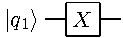
\includegraphics[width=.2\textwidth]{Circuits/X.pdf}
\end{figure}

\textbf{Pauli Y}
\[\begin{pmatrix}
0 & -i \\
i & 0
\end{pmatrix}\]
Flip plus phase difference. Has eigenvalues
\[\ket{+i} = \frac{1}{\sqrt{2}}\begin{pmatrix}1\\i\end{pmatrix} \qquad
\ket{-i} = \frac{1}{\sqrt{2}}\begin{pmatrix}1\\-i\end{pmatrix}
\]

\begin{figure}[h]
    \centering
    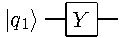
\includegraphics[width=.2\textwidth]{Circuits/Y.pdf}
\end{figure}

\textbf{Pauli Z}
\[\begin{pmatrix}
1 & 0 \\
0 & -1
\end{pmatrix}
\]
Add a phase difference to the $\ket{1}$ state. Eigenvalues are the computaitonal states.

\begin{figure}[h]
    \centering
    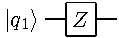
\includegraphics[width=.2\textwidth]{Circuits/Z.pdf}
\end{figure}

\textbf{Phase Gate $R_{\theta}$}
\[\begin{pmatrix}
1 & 0 \\
0 & e^{i\theta}\\
\end{pmatrix}\]

\textbf{CNOT}
\[\begin{pmatrix}
1 & 0 & 0 & 0 \\
0 & 1 & 0 & 0 \\
0 & 0 & 0 & 1 \\
0 & 0 & 1 & 0 \\
\end{pmatrix}
\]
Flips the target qubit, conditioned on the control qubit.

\begin{figure}[h]
    \centering
    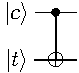
\includegraphics[width=.2\textwidth]{Circuits/cnot.pdf}
\end{figure}

\textbf{SWAP}
\[\begin{pmatrix}
1 & 0 & 0 & 0 \\
0 & 0 & 1 & 0 \\
0 & 1 & 0 & 0 \\
0 & 0 & 0 & 1 \\
\end{pmatrix}\]
Swap qubits 1 and 2.

\begin{figure}[h]
    \centering
    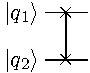
\includegraphics[width=.2\textwidth]{Circuits/swap.pdf}
\end{figure}

\textbf{Hadamard}
\[\frac{1}{\sqrt{2}}\begin{pmatrix}
1 & 1 \\
1 & -1 \\
\end{pmatrix}\]
Rotates between the equator ($\ket{+,-}$) and poles ($\ket{0,1}$) of the Bloch sphere.

\begin{figure}[!h]
    \centering
    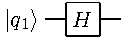
\includegraphics[width=.2\textwidth]{Circuits/h.pdf}
\end{figure}

\subsubsection*{No Cloning}
This is a fundamental theroem of quantum information and a consequence of linearity of quantum mechanics.
Consider a `cloning' unitary $U$ such that
\begin{align}
    U(\ket{0}\otimes\ket{0}) &= \ket{0}\otimes\ket{0} \\
    U(\ket{1}\otimes\ket{0}) &= \ket{1}\otimes\ket{1} \\
\end{align}
Then we might expect to clone an arbitrary qubit state $\ket{\psi} = \alpha\ket{0} + \beta\ket{1}$. But,
\begin{align}
    U(\alpha\ket{0}\otimes\ket{0} + \beta\ket{1}\otimes\ket{0}) &= \alpha\ket{00} + \beta\ket{11}\\
    &\neq \ket{\psi}\otimes\ket{\psi}
\end{align}
as
$\ket{\psi}\otimes\ket{\psi} = \alpha^{2}\ket{00}+\alpha\beta(\ket{01}+\ket{10})+\beta^{2}\ket{11}$
\section{Universal Computing}

We can conceptualise a computation as a boolean function $f : \{0,1\}^{n} \rightarrow \{0,1\}^{m}, n\geq m$, and this operation can be broken up into a circuit if there exist a sequence of one- and many-qubit gates $U_{i}$ such that
\[U_{n}U_{n-1}\cdots U_{1}\ket{\psi_{0}} = \ket{\psi_{out}}\]
where $\ket{\psi_{0}}$ and $\ket{\psi_{out}}$ are computational states belonging to $\mathbb{C}^{n}$ and $\mathbb{C}^{m}$ respectively.

If $n > m$, then the computation is said to be irreversible. The Landauer principle states that there is a thermondynamic cost $k_{B}T \ln_{2}$ associated to erasing a bit, and so an irrevesrible circuit generates $(n-m)k_{B}T\ln_{2}$ of energy.

Reversible computation, clasically, is achieved by adding additional ancillae bits, and using the Toffoli or `CCNOT' gate.
\begin{equation}
    \begin{pmatrix}
        1 & 0 & 0 & 0 & 0 & 0 & 0 & 0\\
        0 & 1 & 0 & 0 & 0 & 0 & 0 & 0\\
        0 & 0 & 1 & 0 & 0 & 0 & 0 & 0\\
        0 & 0 & 0 & 1 & 0 & 0 & 0 & 0\\
        0 & 0 & 0 & 0 & 1 & 0 & 0 & 0\\
        0 & 0 & 0 & 0 & 0 & 1 & 0 & 0\\
        0 & 0 & 0 & 0 & 0 & 0 & 0 & 1\\
        0 & 0 & 0 & 0 & 0 & 0 & 1 & 0\\
    \end{pmatrix}
\end{equation}
It can be shown that this gate is universal for classical computation, meaning with enough bits and a sequence of Toffoli's any classical computation can be implemented.

It turns out that, for quantum computation, we only need to add the Hadamard gate to achieve universal computation. This makes it clear that quantum computing is an extension of the classical, and namely that $P \subseteq BQP$.

\subsubsection*{The Solovay-Kitaev Theorem}
While the set $\{ H, CNOT\}$ is one example, there are many different universal sets, some of which are `overcomplete'. Examples include $\{\text{All Single Qubit Gates},CNOT\}$ and $\{CNOT,H, R_{\frac{\pi}{4}}\}$.

The Solovar-Kitaev Theorem defines what it means for a set of gates to be `universal' for quantum computing.

A set of $t$ normalised, unitary matrices $\{U_{i}\}$ is an $\epsilon$-approximation of a Unitary $U$ if
\begin{align}
\| U - U_{t}U_{t-1}\cdots U_{1}\| \leq \epsilon
\end{align}
where $\|U\| \equiv \max \frac{\| U \ket{\psi}\|}{\|\ket{\psi}\|}, \|\ket{\psi}\| \equiv \sqrt{\braket{\psi}{\psi}}$.

The Solovay-Kitaev theorem states that a set of gates is universal if it can $\epsilon$ approximate any Unitary. The theorem also states that any universal set is $\epsilon$-equivalent to each other, meaning that any `Quantum speedup' can be achieved irrespective of our choice of gates.
\section{The Deutsch-Jozsa Algorithm}
This is the protoypical quantum algorithm, demonstrating how a technique called phase-kickback, in combination with superposition, can be used to significantly reduce the `query complexity' of a problem.

Consider a function $f : \{0,1\}^{n} \rightarrow \{0,1\}$. We are given a black box or `oracle' that can evaluate this function for any input. We want to characterise if the function is `balanced' (outputs $0$ for half the inputs or $1$ for the other half), or `constant' (output always $0$ or $1$). How many times do we have to query the oracle to find out?

Clasically, we can show that for $N=2^{n}$ possible inputs, we need at least $\frac{N}{2} + 1$ queries. But quantum algorithms require only $1$!

\subsubsection*{Quantum Parallelism}
Consider a `register' of $n$ qubits, all initialised in the $\ket{0}$ state. We can then consider applying an $n$-fold Hadamard to each of states $H^{\otimes n}\ket{00\cdots0}$. An $n$-fold Hadamard on superposition of binary strings $\ket{x}$ has the effect
\begin{equation}
    H^{\otimes n}\ket{x} = \frac{1}{\sqrt{2^{n}}}\sum_{y}(-1)^{x\cdot y}\ket{y}
\end{equation}
where
\[x\cdot y \equiv x_{1}\wedge y_{1}\oplus x_{2}\wedge y_{2}\oplus \cdots \oplus x_{n}\wedge y_{n} .\]

For the state $\ket{0}^{\otimes n}$, this initialises the register in a uniform superpostion of all binary strings $x\in\{ 0,1\}^{n}$
\[H^{\otimes n}\ket{00\cdots0} = \frac{1}{\sqrt{2^{n}}}\sum_{x}\ket{x}\]
often denoted simply $\ket{x}$.

To perform reversible computing, like in the classical case, we need additional qubits to keep track of the outputs. If we consider a second register $\ket{0}^{\otimes m}$, we can construct an oracle gate $\hat{O}_{f}$ for a function $f:\{0,1\}^{n}\rightarrow\{0,1\}^{m}$ such that:
\begin{equation}
    \hat{O}_{f}(\ket{x}\otimes\ket{00\cdots 0}) = \frac{1}{\sqrt{2^{n}}} \sum_{x}\ket{x}\otimes\ket{0\oplus f(x)}.
\end{equation}
Effectively, we now have a superposition of the inputs, and the evaluation of the function for each one. This ability to evaulate the oracle for all inputs in a single query is commonly reffered to as Quantum Parallelism.

\subsubsection*{The Algorithm}
The Deutsch-Jozsa algorithm is the name given to the generalisation of this constant/balanced problem for $n$-bit input strings; the Detusch algorithm refers specifcally to the $n=2$ case.

In this algorithm, the second register is instead intialised into the $\ket{-} = \frac{1}{\sqrt{2}}(\ket{0} + \ket{1})$ state.

If the function $f(x)$ evaluates to $1$, then the second register becomes (dropping normalisation):
$\ket{0\oplus 1} - \ket{1\oplus 1} = \ket{1} - \ket{0} = -\ket{-}$
i.e that state picks up a $\pi$ phase.

We then apply a set of Hadamards to the first register, and we can throw away the second register
\begin{align}
    &\sum_{x} H^{\otimes n}\ket{x}\otimes (-1)^{f(x)}\\
    &= \sum_{y}(\sum_{x}(-1)^{f(x)+x\cdot y}\ket{y}) \\
    &= \begin{cases}
        \pm \ket{0}^{\otimes n} & \quad \text{consntant} \\
        \ket{\phi} \neq \ket{0}^{\otimes n} & \quad \text{balanced}
       \end{cases}
\end{align}
To evaluate, we simply need to read out each of the qubits in the first register. If we encounter a $\ket{1}$, we know the function was balanced, otherwise it was constant.

This algorithm is deterministic. Not only that, but it requires only a linear number of Hadamard gates and single oracle query. It has been shown that any boolean oracle can be implemented in a polynomial number of gates, and so this algorithm is computationally efficient.

\begin{figure}[h]
    \centering
    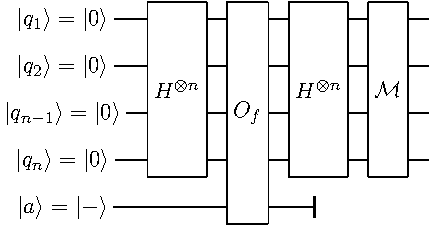
\includegraphics[width=.4\textwidth]{Circuits/dj.pdf}
    \caption{Simplified Circuit for the Deutsch-Jozsa algorithm.}
    \label{fig:djalgo}
\end{figure}

\hrulefill

\textbf{Aside: Boolean Functions and Quantum Circuits}
A boolean function $f : \{0,1\}^{n}\rightarrow\{0,1\}^{m}$ has an `algorithm', which describes how to create a family of circuits $C$ that can evaluate the function for different input sizes $n$. This algorithm is efficient if these circuits have a size that scales polynomially or less with $n$. The circuits are typically represented as acyclic graphs using irreversible operations AND, NOT and OR, along with the FANOUT gate.

These circuits have a reversible implementation, as these elementary operaitons can all be approximated using a sequence of Toffoli gates with enough ancillae bits.

If we consider an archetypal operation e.g. modulo addition, then such a circuit will need $n$ bits to define the Modulo, $n$ for input $x$ and $n$ for input $y$. However, the ouput is only $n$ bits, and so a reversible example must have an additional $n$ `worker' bits $w$, such that the inputs are left unchanged and the worker bits contain the result of the computation.

Generally, for a function $f : \{0,1\}^{n}\rightarrow\{0,1\}^{m}$ with an irreversible circuit $C$, there exists a reversible circuit $R$ with $n$ input bits and $l$ ancilla bits, which gives an output with $m$-data bits and $n+l-m$ `garbage' bits.

This gives a template to implement an oracle; with an additional $m$ `readout' bits, the result can be mapped to these bits with a sequence of CNOTs, and then the inverse operation $R^{-1}$ applied to restore the input and the ancillae.

\hrulefill

\section{Hidden Subgroup Problems}

The Hidden Subgroup Problem is a general state of a class of computational problem. A certain case of these problems, which are clasically known to be in NP, can be solved in polynomial time with a quantum algorithm.

\subsubsection*{Formal Statement}
For a group $G$ and a subgroup $H : \vert H\vert \leq \vert G\vert$, we say that a function $f: G\rightarrow X$ onto the set $X$ `hides the group' $H$ if $\forall g_{1},g_{2}\in G, f(g_{1})=f(g_{2}) \leftrightarrow g_{1}H=g_{2}H$. Equivalent, we say that $f$ is constant within the cosets of $H$.

Given such a function $f$, implemented as an oracle using $O(\log\vert G\vert + \log\vert X\vert)$ bits, how many queries are required to determine a generating set for $H$?

\subsection*{Simons's Problem}
Simon's Problem is an example of the Hidden Subgroup problem, similar to the Deutsch-Jozsa problem. In this case, the gidden group is a single element $s\in\mathbb{Z}_{2}^{N}$, the group of $N$ bit binary strings.

We are given a binary function $f:\{0,1\}^{n}\rightarrow\{0,1\}^{n}$, with the `promise' that it is periodic with period $s$. Namely, for two string $x,y\in\mathbb{Z}_{2}^{n}$,
\begin{equation}
    f(x)=f(y)\implies x\oplus y = s \implies y = x\oplus s\,.
\end{equation}

The initial step of the algorithm is idetical to the Deutsch-Jozsa algorithm; a set of $n$ data qubits are initialised in a coherent superposition of all inputs, and an oracle is acted on the $n$ data qubits and $n$ ancillae to give the state
\begin{equation}
    \frac{1}{\sqrt{2^{n}}}\sum_{x}\ket{x}\ket{f(x)}
\end{equation}
which can be written as a sum over the range of the function $f$ and the hidden group $s$ as
\[\frac{1}{\sqrt{2^{n}}}\sum_{r\in R}(\ket{x}+\ket{x\oplus s})\ket{r}\]

We then apply a second set of Hadamard operations on the first register, and perform a computational basis measurement on the first register. The propbability of obtaining a given string $y$ on readout is then given by
\begin{equation}
    \|\frac{1}{2^{n}}\sum_{r\in R}((-1)^{x\cdot y}+(-1)^{(x\oplus s)\cdot y})\ket{r}\|^{2}
\end{equation}
which gives
\begin{equation}
P(y) = \begin{cases}
2^{-(n-1)} & \quad \text{if} \, s\cdot y = 0\\
0 & \quad \text{if} \, s\cdot y = 1
\end{cases}
\end{equation}
Or, if $s=0$, this is equal to a uniform superpositon over all possible strings.

\begin{figure}
    \centering
    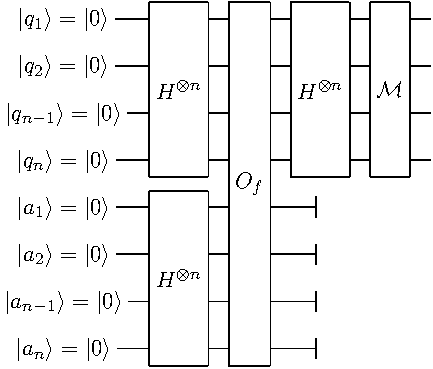
\includegraphics[width=.4\textwidth]{Circuits/simons.pdf}
    \caption{Simplified Circuit for Simon's Algorithm}
\end{figure}

Determing $s$ then requires an iteration of this algorithm to generate $n-1$ strings, which is enough to solve for $s\cdot y = 0$.

The problem here is that the string we obtain on readout is random, and so there is a non-zero probability that we obtain a duplicate string on a given round of the algorithm.

For a given run of the algorith, the probability of obtaining $n-1$ linearly independent string is bounded by
\[\prod_{k=1}^{\infty}1-\frac{1}{2^{k}}>\frac{1}{4}\].
If we repeat our $n-1$ trials $4m$ times, then we have a bounded failure probability
\[(1-\frac{1}{4})^{4m}<e^{-m}\]
which, for $m = 10$, is $\frac{1}{20000}$. Thus, with a linear number of queries, we can find $s$.

\subsection*{Quantum Fourier Transform}
Before discussing other instances of the HSP, we will consider in detail the Quantum Fourier Transform, a key element of these algorithms.

The general statement of a fourier transform is that it takes an input vector of $N$ complex numbers $x$, and transforms it onto a vector $y$ such that
\begin{equation}
    y_{k} \equiv \frac{1}{\sqrt{N}}\sum_{j=0}^{N-1} x_{j}e^{2\pi i j k / N}
\end{equation}
Quantum mechanically, this corresponds to a change of basis such that
\[\ket{j}\rightarrow \frac{1}{\sqrt{N}}\sum_{k=0}^{N-1}e^{2\pi i j k / N}\ket{K}\]
We can write $e^{2\pi i j k / N}$ as the Nth root of unity, $\omega_{N}^{i\times j}$, and write the Fourier transform as $F_{N}$ as a matrix $[F_{N}]_{i,j} = \omega_{N}^{i \times j}$, noting that $\omega_{N}^{M} = \omega_{N}^{M \text{mod} N}$ for $M>N$. This matrix is unitary.

We can write the action of the QFT on a computation state $\ket{x_{1}x_{2}\cdots x_{n}}$
\begin{equation}
    QFT\ket{x} = \frac{(\ket{0}+e^{2\pi i 0. x_{n}}\ket{1})\otimes\cdots(\ket{0}+e^{2\pi i 0. x_{1}x_{2}\cdots x_{n}}\ket{1})}{2^{\frac{n}{2}}}
\end{equation}
where $0.x = \frac{x}{2^{\vert x \vert}}$.


The quantum fourier transform $F_{N}$ can be efficiently decomposed into the Hadamard gate, which is equivalent to $F_{2}$, controlled-phase gates and the transform $F_{N-1}$ The phase gates are denoted $R_{k}$ where
\[R_{k}=\begin{pmatrix}1 & 0 \\ 0 & e^{2\pi i /2^{k}}\\\end{pmatrix}.\] An example is shown below for $F_{3}$.

\begin{figure}[h]
    \centering
    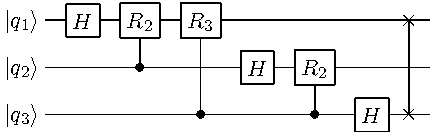
\includegraphics[width=.5\textwidth]{Circuits/F3.pdf}
    \caption{Quantum Circuit for the $F_{3}$ QFT}
\end{figure}

More generally, we consider a `flipped' QFT $\tilde{F_{n}}$ acting on a state $\ket{\tilde{x}}=\ket{x_{n}x_{n-1}\cdots x_{1}}$
\begin{equation}
    \tilde{F_{n}}\ket{\tilde{x}} =
    \frac{1}{\sqrt{2^{n}}}\sum_{i=1}^{2^{n}}\omega_{2^{n}}^{jk}\ket{x_{1}x_{2}\cdots x_{n}}
\end{equation}

Then we can write $\tilde{F_{n}}$ as $\tilde{F_{n-1}}$, and a squence of controlled phase gates and a final Hadamard. A simplified circuit, skipping many qubits, is shown in the figure below. $F_{n}$ can be obtained from $\tilde{F}_{n}$ by adding a squence of swap gates to change the order of the bits.

\begin{figure}[h]
    \centering
    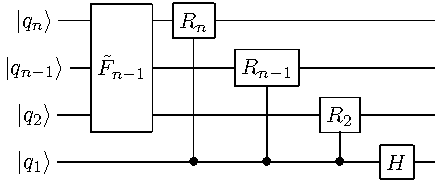
\includegraphics[width=.5\textwidth]{Circuits/Fm.pdf}
\end{figure}

From the circuit above and the circuit for $F_{3}$, we can build any QFT gate using $\frac{n(n+1)}{2}$ phase gates and Hadamards, and a final $\frac{n}{2}$ swap gates, meaning it can be achieved in $\Theta (n^{2})$ gates.

\subsection*{Phase Estimation}
Consider an oracle implementing some large unitary operation $U$. We know that this $2^{n}\times2^{n}$ matrix has $2^{n}=N$ orthonormal eigenvectors with associated eigenvalues $e^{2\pi i \theta_{i}}$. Given a state $\ket{\psi}$ that is promised to be an eigenvector of $U$, can we find its eigenvalue phase $\theta_{i}$?

We begin with two registers. The first register has $n$ qubits, the number of which limits our precision of the estimate for $\theta_{i}$, and the second register stores $\ket{\psi}$. We seek to implement a channel $\Lambda: \ket{k}\otimes\ket{\psi} \rightarrow \ket{k}\otimes U^{k}\ket{\psi}$.

We then perform the usual trick of initialising the first reigster in a coherent superposition of all $N=2^{n}$ inputs, and applying this operation. We can throw away the state $\ket{\psi}$ as it is a product with the result, leaving
\begin{equation}
    \frac{1}{\sqrt{2^{n}}}\sum_{k=0}^{2^{n} -1}e^{2\pi i k \theta_{i}}\ket{k}
\end{equation}

\subsubsection*{Case 1: $\theta_{i} = \frac{j}{2^{n}}$}
In this case, our phase can be exactly represented in the bits we use for the first register. The state we have reduces to

\begin{equation}
    \frac{1}{\sqrt{2^{n}}}\sum_{k=0}^{2^{n} -1}e^{2\pi i k \theta_{i}}\ket{k} =
    \frac{1}{\sqrt{2^{n}}}\sum_{k=0}^{2^{n} -1}\omega^{jk}\ket{k}
\end{equation}
where $\omega$ is the $2^{n}$th root of unity. Thus, we need simply act the inverse QFT $F_{n}^{*}$, and we obtain a computational state $\ket{x_{1}x_{2}\cdots x_{n}}=\ket{x}$, where $\theta_{i}=0.x$!

\subsubsection*{Case 2: $\theta_{i}\neq \frac{j}{2^{n}}$}

If $\theta_{i}$ cannot be exactly represented in $n$ bits, then we consider the best approximation $b:\theta_{i}-\frac{b}{2^{n}} = \delta \in[0,2^{-n}]$. In this case, applying $F^{*}_{n}$ gives the state
\begin{equation}
    \frac{1}{\sqrt{2^{n}}}\sum_{k,l=0}^{2^{n} -1}
    e^{-2\pi i k l /2^{n}} e^{2\pi i \theta_i k}\ket{l}
\end{equation}
The amplitude of a state $\ket{(b+l)\mod 2^{n}}$ can be shown to equal
\[\frac{1}{2^{n}}(\frac{1-e^{2\pi i (2^{n}\delta - l)}}{1-e^{2\pi i (\delta - l/2^{n})}})\]

We can show that the probability of an output string $m:\vert m-b\vert > e$, the error tolerance, is $\frac{1}{2(e-1)}$. Thus, to approximate $\theta_{i}$ to $t$ bits with $p_{success}\geq 1-\epsilon$ requires $n = t + [\log(2+\frac{1}{2\epsilon})]$ qubits.

Assuming we don't know an eigenstate of $U$, this can be shown to work for a state $\ket{\psi}=\sum_{n}c_{n}\ket{u_{n}}$, giving the associated eigenvalue $\theta_{n}$ with probability $\vert c_{n}\vert^{2}$.
\subsection*{Order Finding}
Order finding is a number theoretic problem that is most commonly studied in the context of prime factorisation, namely finding two prime numbers $p,q$ such that $N=pq$.

Given a number N and the range of position integers below it $\mathbb{Z}_{N}=\{0,1,2\cdots N\}$, we define $\mathbb{Z}_{N}^{*}=\{a\in \mathbb{Z}_{N} : gcd(a,N) = 1\}$. This, combined with modulo multplication, forms a group such that there is one unique element $b: ab\mod N = 1$. Each element $a$ also has an order, $r>0,\in \mathbb{Z}_{N} : a^{r}\mod N = 1$. This order $r=\vert \mathbb{Z}_{N}^{*}\vert$.

Clasically, finding this order is computationally hard. However it turns out this problem can be reduced efficiently to solving  a phase estimation problem, which as we showed requires a single quantum oracle query.

We consider a reversible transformation
\[\Lambda_{n}(M_{a})\ket{k}\ket{x}=\ket{k}M_{a}^{k}\ket{x}= \ket{k}\ket{a^{k}x\text{mod} N}\]
which has eigenvectors
\begin{equation}
    \ket{\psi_{j}} = \frac{1}{\sqrt{r}}\sum_{l=0}^{r}\omega_{r}^{-jl}\ket{a^{l}\text{mod} N}
\end{equation}
and associated eigenvalues $e^{\frac{2\pi i k}{r}}$. This makes it clear that, by finding the eigenvalue of such a state using phase estimation, we can then obtain $r$.

The operation above can be constructed via `modular exponentiation', a classical boolean algorithm. We can use the method described at the end of Section~3 to calculate $\ket{a^{k}\text{mod}N}$, and then multiply this result by the second register, before applying the inverse operation to restore inputs and ancillae used. This requires $O(n^{3})$ operations to complete, as $\ket{k}$ has $n$ bits and for each bit we require $O(n^{2})$ operations to calculate $x^{k_{l}2^{l-1}}\text{mod}N$ for each bit of $k$.

For $n$ qubits we have some $j\in\{0,1\cdots 2^{n}\}$, such that $r \approx \frac{2^{n}}{j}+\frac{1}{2}$. We want to be within $\epsilon$ of $r$, which will give the correct $r$ by rounding to the nearest integer if $\vert\epsilon\vert \leq \frac{1}{2N^{2}}$, which in turn implies $n= 2\log(N)$.

Alternatively, we can use the fact that $\frac{k}{r}$ must be rational, as it is the product of two integers, we can obtain $r$ without requiring knowledge of $k$. Any given rational number $x$ has an expression as a sequence of integers $[a_{0},a_{1},\cdots a_{m}]$ such that
\begin{equation}
    x = a_{0}+\frac{1}{a_{1}+\frac{1}{a_{2}+\frac{1}{a_{3}+\cdots}}}
\end{equation}

And so, we can use the continued fractions algorithm to identify this expansion and thus obtain $\frac{k}{r}$, in $O(n^{3})$ operations.

How can we obtain these (mutually orthogonal) eigenstates of the modular exponentiation operator? We can exploit that fact that
\begin{equation}
    \ket{11\cdots 1} = \frac{1}{\sqrt{r}}\sum_{j=0}^{r-1}\ket{\psi_{j}}
\end{equation}
and so after performing the phase-estimation procedure, when reading out the first register we pick one phase $\theta_{j}$ associated to $\ket{\psi_{j}}$ uniformly at random.

Given that we can make the error of phase estimation arbitrarily small for a small increase in the circuit size, the main source of error is if $j$ and $r$ have a common factor, and so the algorithm will return $r'$ which is not necessarily $r$. However, the probability that $j$ and $r$ are co-prime is very high, and in these intances the continued fractions method is guaranteed to work.

This is because there are at least $\frac{r}{2\log r}$ prime  numbers less than $r$, meaning the probability $j$ is prime is $> \frac{1}{2\log r} > \frac{1}{2 n}$, and so $2 n$ repetitions will suffice to find the correct $r$. Another method which also requires an additional $O(n)$ repetitions, is to repeat the procedure to find the order of $a'=(a^{r'})\text{mod}N$.

Alternatively, we can take the trials $r_{i}$ froma given run of the algorithm, and as long as the $s_{i}$ do not have common factors, we can find $r$ from the lowest common multiples of $r_{i}$. The probability this succeeds in two trials is at least $\frac{1}{4}$.

The total cost of this procedure is then $O(n^{3})$, most of which is consumed during the modular exponentiation step.

\subsection*{Shor's Algorithm}
Shor's algorithm can achieve prime factorisation, a problem clssicaly solvable only in sub-exponential time, also in $O(n^{3})$ operations, an exponential speed up.

This is because there exists a `reduction' of prime factorisation to the problem of order finding, and we can use the above algorithm to solve the problem in $O(n^{3})$.

For an integer input $N$, the result is easy if $N$ is prime or a `prime power' $p^{k}$, or if $N$ is even. We can consider a recursive algorithm that keeps going until we find some non-trivial case, and which then outputs two factors $N=pq$.
The procedure can be repeated for these factors, to find all the prime factors of any input $N$.

Consider picking a random number $a\in{2,3,\cdots ,N-1}$. This number has a unique order in $\mathbb{Z}_{N}^{*}$, such that $N$ is dived by $a^{r}-1$ (we write $N\vert a^{r}-1)$).

This implies that $N\vert(a^{\frac{r}{2}}-1)(a^{\frac{r}{2}}+1)$. We are only interested if $x^{\frac{r}{2}}\text{mod} N\neq -1$, and if $r$ is even.

Assuming this isn't the case, computing the greatest common denominator of $a^{\frac{r}{2}}\pm1$ and $N$ gives a non-trivial factor.

We can thus proceed by picking a number $a$ at random, and trialing the algorithm. The probability of success for a given run of the order-finding subroutine is $\frac{1}{2}$. Finding the greatest common denomintaor is possible classically in $O(n^{2})$ gates, and we typically need $O(\log(n))$ repitions, menaing the limiting factor is the $O(n^{3})$ required by the order-finding routine.

\subsection*{Interpreation as a HSP}
All of the algorithms dicussed so far can be interpreted as a Hidden Subgroup problem. For an abelian group, qauntum algorithms can solve the HSP in poly time with respect to the order of the whole group to be searched $\vert G\vert$.

The general procedure is to use the QFT to intialise a uniform superposition of the group elements
\[\frac{1}{\sqrt{\vert G \vert}}\sum_{g}\ket{g}\]
and then apply an oracle which implements the function $f$ hiding the subgroup $H$, giving
\[\frac{1}{\sqrt{\vert G \vert}}\sum_{g}\ket{g}\ket{f(g)}\]

We can rewrite $\ket{f(g)}$ in the Fourier basis
\[\ket{f(g)}=\frac{1}{\sqrt{\vert G \vert}}\sum_{l}
e^{2\pi i l \frac{g}{\vert G\vert}}\ket{\hat{f}(l)}
\]

But as $f$ is constant in the cosets of the subgroup $H$, $\ket{\hat{f}(l)}$ has non-zero amplitude only for the cases
\[\sum_{h\in H}e^{-2\pi l \frac{h}{\vert G\vert}}=\vert H\vert\]
meaning we can apply the inverse QFT to obtain $l$, and from this obtain elements of $H$ sufficient to find a generating set.

While this understnding works for the cases of Phase estimation, or for simpler cases like Deutsch-Jozsa and Simon's problems, it is difficult to conceptualise how it works generally. The key lies in the fact that any finite abelian group is isomorphic to a product of cyclic groups with prime power orders $p_{j}$, such that we can find $l_{j}$ in the expression
\[e^{2\pi i l \frac{g}{\vert G\vert}}=\prod_{j}e^{2\pi i l_{j}\frac{g_{j}}{p_{j}}}\]
from basic phase estimation, and from there obtain $l$ and the group $H$.

\section{Grover's Algorithm}

Grover’s Algorithm is a quantum computing routine broadly described as a `quantum search’. It allows us to search through a dataset to find entries that match a criteria, encoded by a boolean function. This method can be applied to a broad range of problems, including `explicit’ searching, looking for particular records in large databases e.g. web search or real-time processing of financial transactions, or for `implicit’ searching, seeking for example the solution that satisfies an NP-Complete problem e.g. satisfiability, or geometric optimisation problems such as the Travelling Salesman.

Grover's Algorithm requires a pair of gates to perform the search. The first is an oracle, which implements a function $f:\{0,1\}^{n}\rightarrow\{0,1\}$, returning $1$ only if the input `matches' the search criteria. This function could be a polynomial-time verifier for an implicit search problem, or a `comparison' for explicit search.

Using an additional ancilla bit, initialised in the $\ket{-}$ state, we can exploit phase-kickback to mark our solution amongst a coherent superposition of input states.
\begin{equation}
    \hat{O}_{f}\ket{x}\ket{-} = (-1)^{f(x)}\ket{x}\ket{-}
\end{equation}

We then apply a second gate, called the interpreter or diffusion operator, which inverts the amplitudes of a state around the `average'
\[\alpha_{k}' = \langle\alpha\rangle - \delta_{k}\]
where $\delta_{k} = \alpha_{k}-\langle\alpha\rangle$.

The action of these two gates is to `boost' the amplitude of the state that matches the search criteria, and supress the others. By repeating this procedure, we can increase our probability of finding the `true' state by reading out the first register. The diffusion operator is performed applying an n-fold Hadamard after the oracle, phase-shifting any state except $\ket{00\cdots 0}$, before reapplying the Hadamard.

\begin{figure}[h]
    \centering
    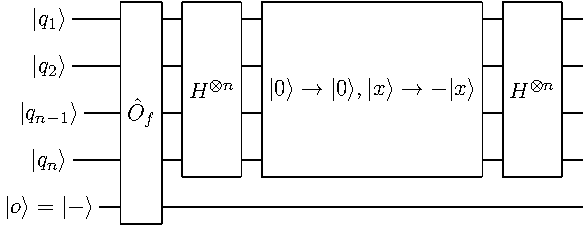
\includegraphics[width=.5\textwidth]{Circuits/grover.pdf}
    \caption{Simplified circuit showing the Grover iteration.}
\end{figure}

Geometrically, we can estimate how many repetitions of the `Grover iteration' we need to maximise the probability of finding a solution to the search problem. Assume there are $M$ matches in a data set of $N$.

We split the space of all computational states into the `target' and `junk' subspaces
\begin{align*}
    \ket{t} &= \frac{1}{\sqrt{M}}\sum_{m\in M}\ket{m} \\
    \ket{\chi} &= \frac{1}{\sqrt{N-M}}\sum_{x\notin m}\ket{x}
\end{align*}
and the intial coherent superposition can be written
\begin{equation}
    \ket{\psi}=\frac{1}{\sqrt{N}}\sum_{x}\ket{x} = \sin(\frac{\theta}{2})\ket{t}+\cos(\frac{\theta}{2})\ket{\chi}
\end{equation}
where $\frac{\theta}{2}=\sin^{-1}(\sqrt{\frac{N-M}{N}})$. Plotting this vector in $\ket{t},\ket{\chi}$ space, the action of the grover iteration is to first flip the vector in $t,\chi$ space around the $\chi$ axis, and then flip this fector around the initial state. The total action is a rotation through an angle $\theta$.

The amplitude of the target states is maximal, then, when we have rotated through to an angle $\frac{\pi}{2}\approx\theta'=\frac{2k+1}{2}\theta$ for $k$ applicaitons of the Grover iteration. This means we need approximately
\begin{equation}
    k=\lfloor \frac{\cos^{-1}(\sqrt{\frac{M}{N}})}{\theta} \rfloor
\end{equation}
applications to maximise the probability of finding a target state.

A simpler bound can be obtained by rearranging the expression above to obtain the upper bound
\begin{equation}
    k \leq \lceil \frac{\pi}{4}\sqrt{\frac{N}{M}} \rceil.
\end{equation}
For $M=1$, this means we need $O(\sqrt{N})$ queries, improving over the $\frac{N}{2}$ searches required for a classical brute force search. This is only a quadratic speedup, rather than the exponential speed up offered by Shor's algorithm, but could be used to

\subsection*{Implicit and Explicit Search}
For an implicit search problem, the oracle gate is simply the circuit that implements the efficient polynomial verifier for the problem. Thus, we expect Grover's algorithm to have an efficient implementation. But what about explicit search problems?

We wish to find the target $\ket{t}$ in the register. Assume it is stored in $l$ bits, and there are $N=2^{n}$ entries. We need four registers then
\begin{itemize}
    \item An $n$ qubit register to hold the index
    \item An $l$ qubit register to hold $t$
    \item An $l$ qubit register to hold `loaded' data
    \item A single qubit to probide phase kickback
\end{itemize}

This method suggests a quantum memory, which would allow us to load superpositions of data in to memory, and to implement the oracle by comparing the loaded data to the target $t$. This would need only $O(\sqrt{N})$ load operations, compared to $O(N)$ clasically.

But, this scheme could also operate with a classical memory, provided we have access to a quantum addressing system. Such a system would need an additional $O(Nn)$ switches.

\subsubsection*{Optimality}
Quantum Search is in fact the optimal algorithm for unstructured search. To illustrate this, consider an initial state $\ket{\psi}$, and an oracle that marks a single target state $x$. We apply a sequence of unitary operations $U_{i}$ and the oracle $O_{x}$ $k$ times
\begin{align*}
  \ket{\psi_{k}^{x}}&=U_{k}O_{x}U_{k-1}\cdots U_{1}O_{x}\ket{psi}\\
  \ket{\psi_{k}} &= U_{k}U_{k-1}\cdots U_{1}\ket{\psi}
\end{align*}

We want to bound the quantity $D_{k}\equiv \sum_{x} \| \psi_{k}^{x}-\psi_{k}\|^{2}$, as the probability of finding the target is better the larger $D$ is. We show that $D$ grows as $k^{2}$, and must be $\Omega
(N)$ to distinguish among $N$ items.

As the maximal difference for the Oracle is $O_{x}\ket{\psi}=-\ket{\psi}$, $D_{k}\leq 4 k^{2}$. Using
$D_{k+1}=\sum_{x} \| O_{x}\psi_{k}^{x} - \psi_{k}\|$, we can show that $ D_{k+1}\leq D_{x} + 4\sqrt{D_{k}}+4$, and thus
\[ D_{k+1}\leq 4(k+1)^{2}.\]

To bound the required size of $D$, we consider the situation $\vert \braket{x}{\psi_{k}^{x}}\vert^{2}\geq\frac{1}{2}$, meaning we are more likely to find the target. We then have
\[\| \psi_{k}^{x}-x\|^{2}\leq 2-\sqrt{2}\]

and thus, defining $E_{k}=\sum_{x}\| \psi_{k}^{x}-x\|^{2}$ and $F_{k} = \sum_{x}\| x- \psi_{k}^{x}-\|^{2}$, we can write
\[
D_{k}\geq E_{k}+F_{k} -2\sqrt{E_{k}F_{k}}
\]
and using $E_{k}\leq(2-\sqrt{2})N,F_{k}\geq(2-\sqrt{2})N$, we can show that to be able to disntinguish $x, D_{k}\geq cN$.

Combining this with the above result gives
\begin{equation}
    k\geq\sqrt{\frac{cN}{4}}
\end{equation}
showing that $O(\sqrt{N})$ is optimal.
% \subsection*{Grover as simulation}
\end{document}
